\documentclass[6pt,a4paper]{article}

\usepackage[frenchb]{babel}
\usepackage{graphicx}
\usepackage{subcaption}
\usepackage{amssymb}
\usepackage{fancyhdr}

\pagestyle{fancy}

\renewcommand{\headrulewidth}{1pt}
\fancyhead[L]{\textbf{RCE2}}
\fancyhead[R]{\textbf{Ail et fines'eirb}}

\renewcommand{\footrulewidth}{1pt}
\fancyfoot[C]{\textbf{page \thepage}}
\fancyfoot[L]{\textbf{Eirspace}}
\fancyfoot[R]{\textbf{23-24}}

\begin{document}

\titlepage
\begin{center}
	\rule{\textwidth}{1pt}

	\vspace{1\baselineskip}

	\Large D\large ebrief du RCE02

	\vspace{1\baselineskip}

	\large Ail et fines'eirb

	\vspace{1\baselineskip}

	\textit{ENSEIRB-MATMECA 23-24}

	\rule{\textwidth}{1pt}
\end{center}


\newpage
\begin{center}
	\tableofcontents
\end{center}


\newpage
\section{\large Stabilité}

\vspace{1\baselineskip}

Il y a \textbf{3} manières pour rendre la fusée stable : 
\begin{itemize}
	\item Réduire la longueur de la fusée
	\item Lester le bas de la fusée
	\item Modifier la forme des ailerons
\end{itemize}

\vspace{1\baselineskip}

Notre fusée pourrait faire \textbf{120cm}. Elle est trop longue.

Pour la rendre stable, on va modifier la forme des ailerons

\vspace{1\baselineskip}

\begin{figure}[h]
	\begin{minipage}[t]{0.45\textwidth}
		\begin{center}
			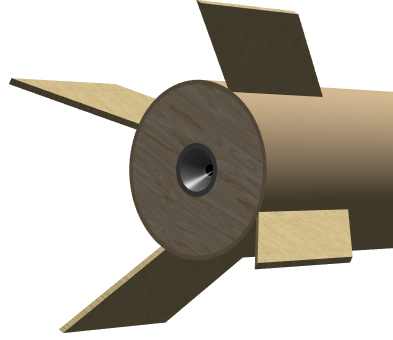
\includegraphics[width=1\textwidth]{pics/ailerons.png}
		\end{center}
		\caption{\small Ailerons actuels}
	\end{minipage}
	\hfill
	\begin{minipage}[t]{0.45\textwidth}
		\begin{center}
			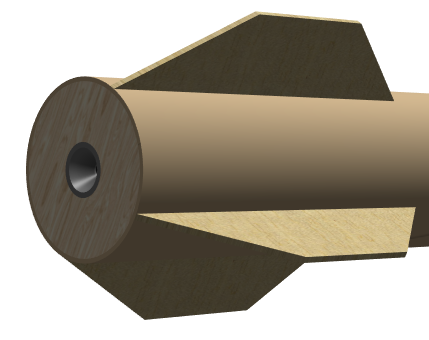
\includegraphics[width=1\textwidth]{pics/ailerons_voulus.png}
		\end{center}
		\caption{\small Ailerons voulus}
	\end{minipage}
\end{figure}

\vspace{1\baselineskip}

La forme des ailerons va rendre la fusée stable. Cette forme reste à être trouvée grâce au \textbf{stabtraj}.

La \textit{figure 2} n'est pas exacte.

\vspace{1\baselineskip}

\section{\large Fixations}

\vspace{1\baselineskip}

Les propulseurs (cette année le \textit{Cesaroni Pandora Pro 24G}) sont réutilisés chaque année.

Ainsi il ne faut \textbf{pas l'endommager}.

\vspace{1\baselineskip}

On va fixer à \textbf{3 endroits} le propulseur :
\begin{enumerate}
	\item Au bas de la fusée avec une \textbf{bague structurelle}
	\item Au milieu du propulseur avec une \textbf{bague structurelle}
	\item En haut de la fusée contre le \textit{camenbert}, qui doit être un peu creu quand même, avec une \textbf{bague structurelle}
\end{enumerate}

\vspace{1\baselineskip}

Pour former un ensemble très solide entre le propulseur et le reste de la fusée, on pourrait créer des \textbf{liaisons encastrement} entre ce dernier et les ailerons.

\vspace{1\baselineskip}

On pourrait pour cela utiliser des \textbf{vis radiales}. Il reste à définir leur positionnement.

\vspace{1\baselineskip}

\section{\large Parachute}

\vspace{1\baselineskip}

On va utiliser une \textbf{bague structurelle} pour fixer le parachute.

\vspace{1\baselineskip}

Il y a une façon de faire spéciale pour ouvrir la trappe, pour que l'air s'engouffre bien dans le compartiment.

\vspace{1\baselineskip}

\section{\large Carte réseau}

\vspace{1\baselineskip}

Il ne faut pas utiliser la fréquence 915Mhz.

Les cartes réseau type \textbf{LoRa} ne sont pas adaptées au type de fréquence autorisé en France.

\vspace{1\baselineskip}

Il faudrait donc utiliser un module \textbf{FPV}, mais la retransmission va être moins puissante.

\vspace{1\baselineskip}

\section{\large Séquenceur}

\vspace{1\baselineskip}

Il ne faut pas dépasser \textbf{5V} pour ne pas griller la carte Arduino.

On utilisera un \textbf{GPIO}.

\vspace{1\baselineskip}

\section{\large Plan de rétroaction}

\vspace{1\baselineskip}

Pour \textbf{fin Mars}:
\begin{itemize}
	\item Finir la conception de la fusée,
	\item Imprimer les camemberts et l'ogive en 3D.
\end{itemize}

\vspace{1\baselineskip}

Pour \textbf{Avril}:
\begin{itemize}
	\item Finir la fusée (sans les expériences),
	\item Finir le stabtraj.
\end{itemize}

\end{document}
